\section{Collimator\_linear: The simple Soller blade collimator}
\label{collimator-linear}\index{Optics!Linear collimator}

\component{Collimator\_linear}{System}{$x_{min}$, $x_{max}$, $y_{min}$, $y_{max}$, $L$, $\delta$ (in deg.)}{}{}

The component {\bf Collimator\_linear}
models a standard linear Soller blade collimator.
The collimator has two identical rectangular openings,
defined like the one in {\bf Slit}. Neutrons not clearing both
openings are ABSORB'ed, see the discussion in \ref{slit}.
The collimating effect is taken care of by employing an ideal
triangular transmission through the collimator, as explained below.
For a more detailed Soller collimator simulation,
taking every blade into accountm , the {\bf Channeled\_guide}
component can be employed, see section~\ref{s:channeled_guide}.

Let $L$ be the length of the collimator blades
and $d$ the distance between them.
Then let $\phi$ be the angle between the
neutron path and the vertical $y-z$ plane along the collimator axis
($\phi$ is also called the {\em horizontal divergence}).
We then define the collimation angle as the maximal allowed
horizontal divergence: $\delta = \tan^{-1}(d/L)$,
see Fig.~\ref{f:collimator}. Neutrons with a horizontal
divergence angle $|\phi| \geq \delta$ will always
hit at least one collimator blade and will thus be ABSORB'ed.
For smaller divergence angles, $|\phi| < \delta$, the fate of the
neutron depends on its exact entry point.
Assuming that a typical collimator has many blades, the
absolute position of each blade perpendicular to the collimator axis
is somewhat uncertain (and also unimportant in most cases).
A simple statistical consideration now shows that the transmission
probability is $T = 1-\tan|\phi|/\tan\delta$.

\begin{figure}
  \begin{center}
    \psfrag{xmin}[c][c]{$x_{\rm min}$}
    \psfrag{xmax}[c][c]{$x_{\rm max}$}
    \psfrag{ymin}[c][c]{$y_{\rm min}$}
    \psfrag{ymax}[c][c]{$y_{\rm max}$}
    \psfrag{delta}[c][c]{$\delta$}
    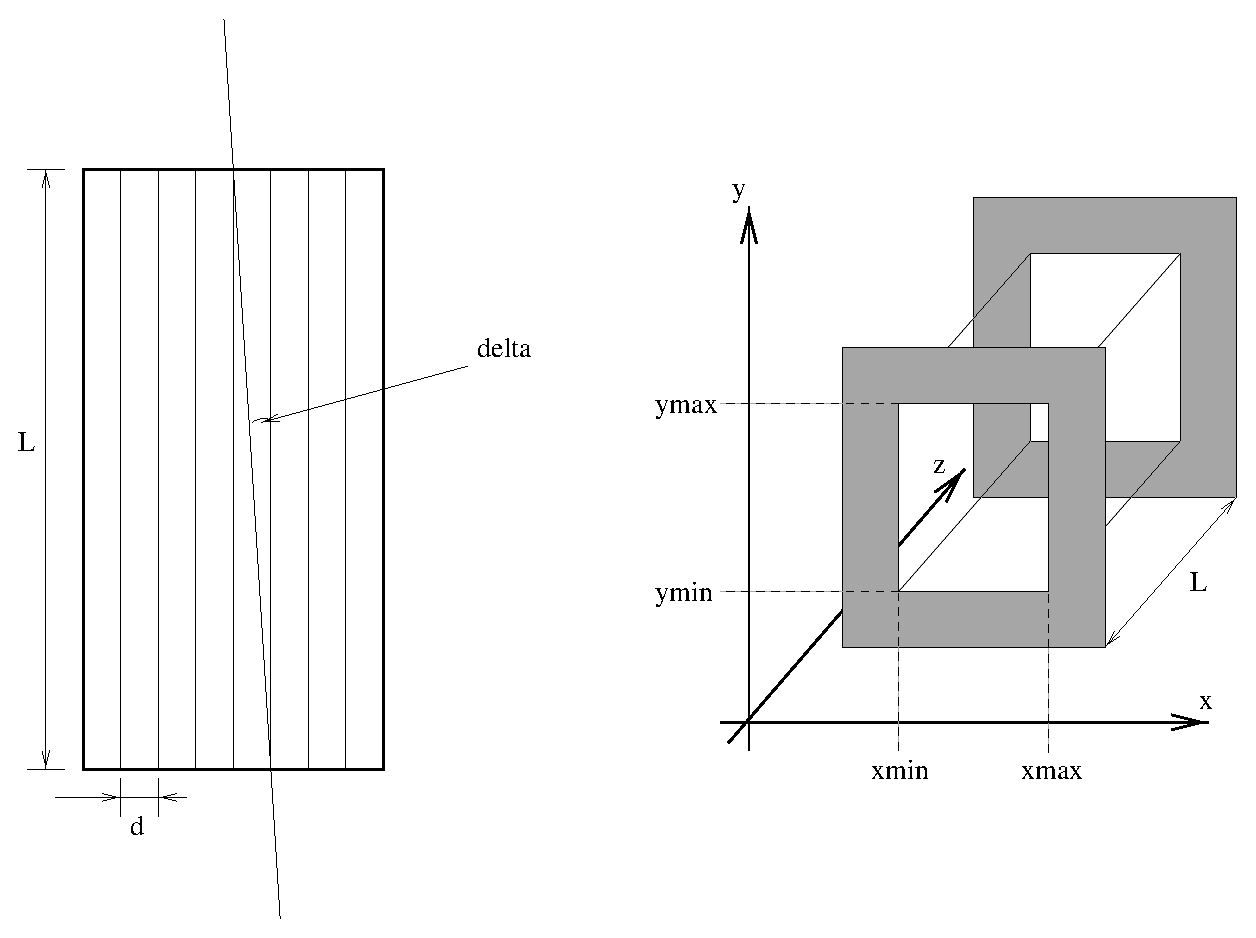
\includegraphics[width=0.9\textwidth]{figures/collimator.eps}
  \end{center}
\caption{The geometry of a simple Soller blade collimators:
The real Soller collimator, seen from the top (left),
and a sketch of the component {\bf Soller} (right).
The symbols are defined in the text.}
\label{f:collimator}
\end{figure}

We simulate the collimator by transmitting all neutrons with
$|\phi| < \delta$, but adjusting their weight with the amount
\begin{equation}
\pi_i = T = 1-\tan|\phi|/ \tan\delta ,
\end{equation}
while all others are discarded by the kernel call ABSORB.
If $\delta=0$, the collimating effect is disabled,
so that $\pi_i = 1$ whenever the neutron clears the two apertures.
